%        File: figs.tex
%     Created: Fri May 02 05:00 pm 2014 E
% Last Change: Fri May 02 05:00 pm 2014 E
%
\documentclass[a4paper]{report}
\usepackage{algorithm2e}
\usepackage{graphicx}
\usepackage{amsmath}
\usepackage{cite}
\usepackage{framed, color}
\usepackage{soul}
\definecolor{shadecolor}{rgb}{.93,.93,.93}
\definecolor{blu}{rgb}{0,0,1}
\newcommand{\td}[1]{{\color{blu}\hl{TODO: #1}}}
\definecolor{shadecolor}{rgb}{.93,.93,.93}
\usepackage{amssymb}
\usepackage{mathrsfs}
\usepackage{gensymb}
\setlength{\parindent}{1cm}
\setlength{\parskip}{1cm plus2mm minus2mm}
\usepackage[hmargin=1.4cm,vmargin=1.4cm]{geometry}
\setlength{\parindent}{0cm}
\setlength{\parskip}{4mm plus1mm minus1mm}
\usepackage[colorlinks=true,urlcolor=blue]{hyperref}

\begin{document}
\begin{table}[t]
\centering
	\begin{tabular}{ l  l  l }
		\hline                       
		Treatment & Funder & Priming Image Set	\\ 
		\hline                       
		$\textsc{ambg}$ & None & Ambiguous\\
		$\textsc{cult}_{img}$ & None & Cultural\\
		$\textsc{cult}_{fund}$ & Cultural & Cultural\\
		$\textsc{cult}_{fund,img}$ & Cultural & Cultural\\
		$\textsc{ingr}_{img}$ & None & Ingredients\\
		$\textsc{ingr}_{fund}$ & Nutritional & Ingredients\\
		$\textsc{ingr}_{fund, img}$ & Nutritional & Ingredients\\
		\hline  
	\end{tabular}

%\begin{addmargin}[11em]{11em}
%	\vspace{2mm}
%	$^a$\footnotesize{The full funder names used were ``The Glodal Foundation
%		for Cultural Recognition'' and ``The National Foundation for 
%		Nutritional Awareness''.}
%\end{addmargin}

	\caption{Workers were uniformly randomly
		assigned to one of the treatments listed above.}
	\label{table:1}
\end{table}

\begin{figure}
	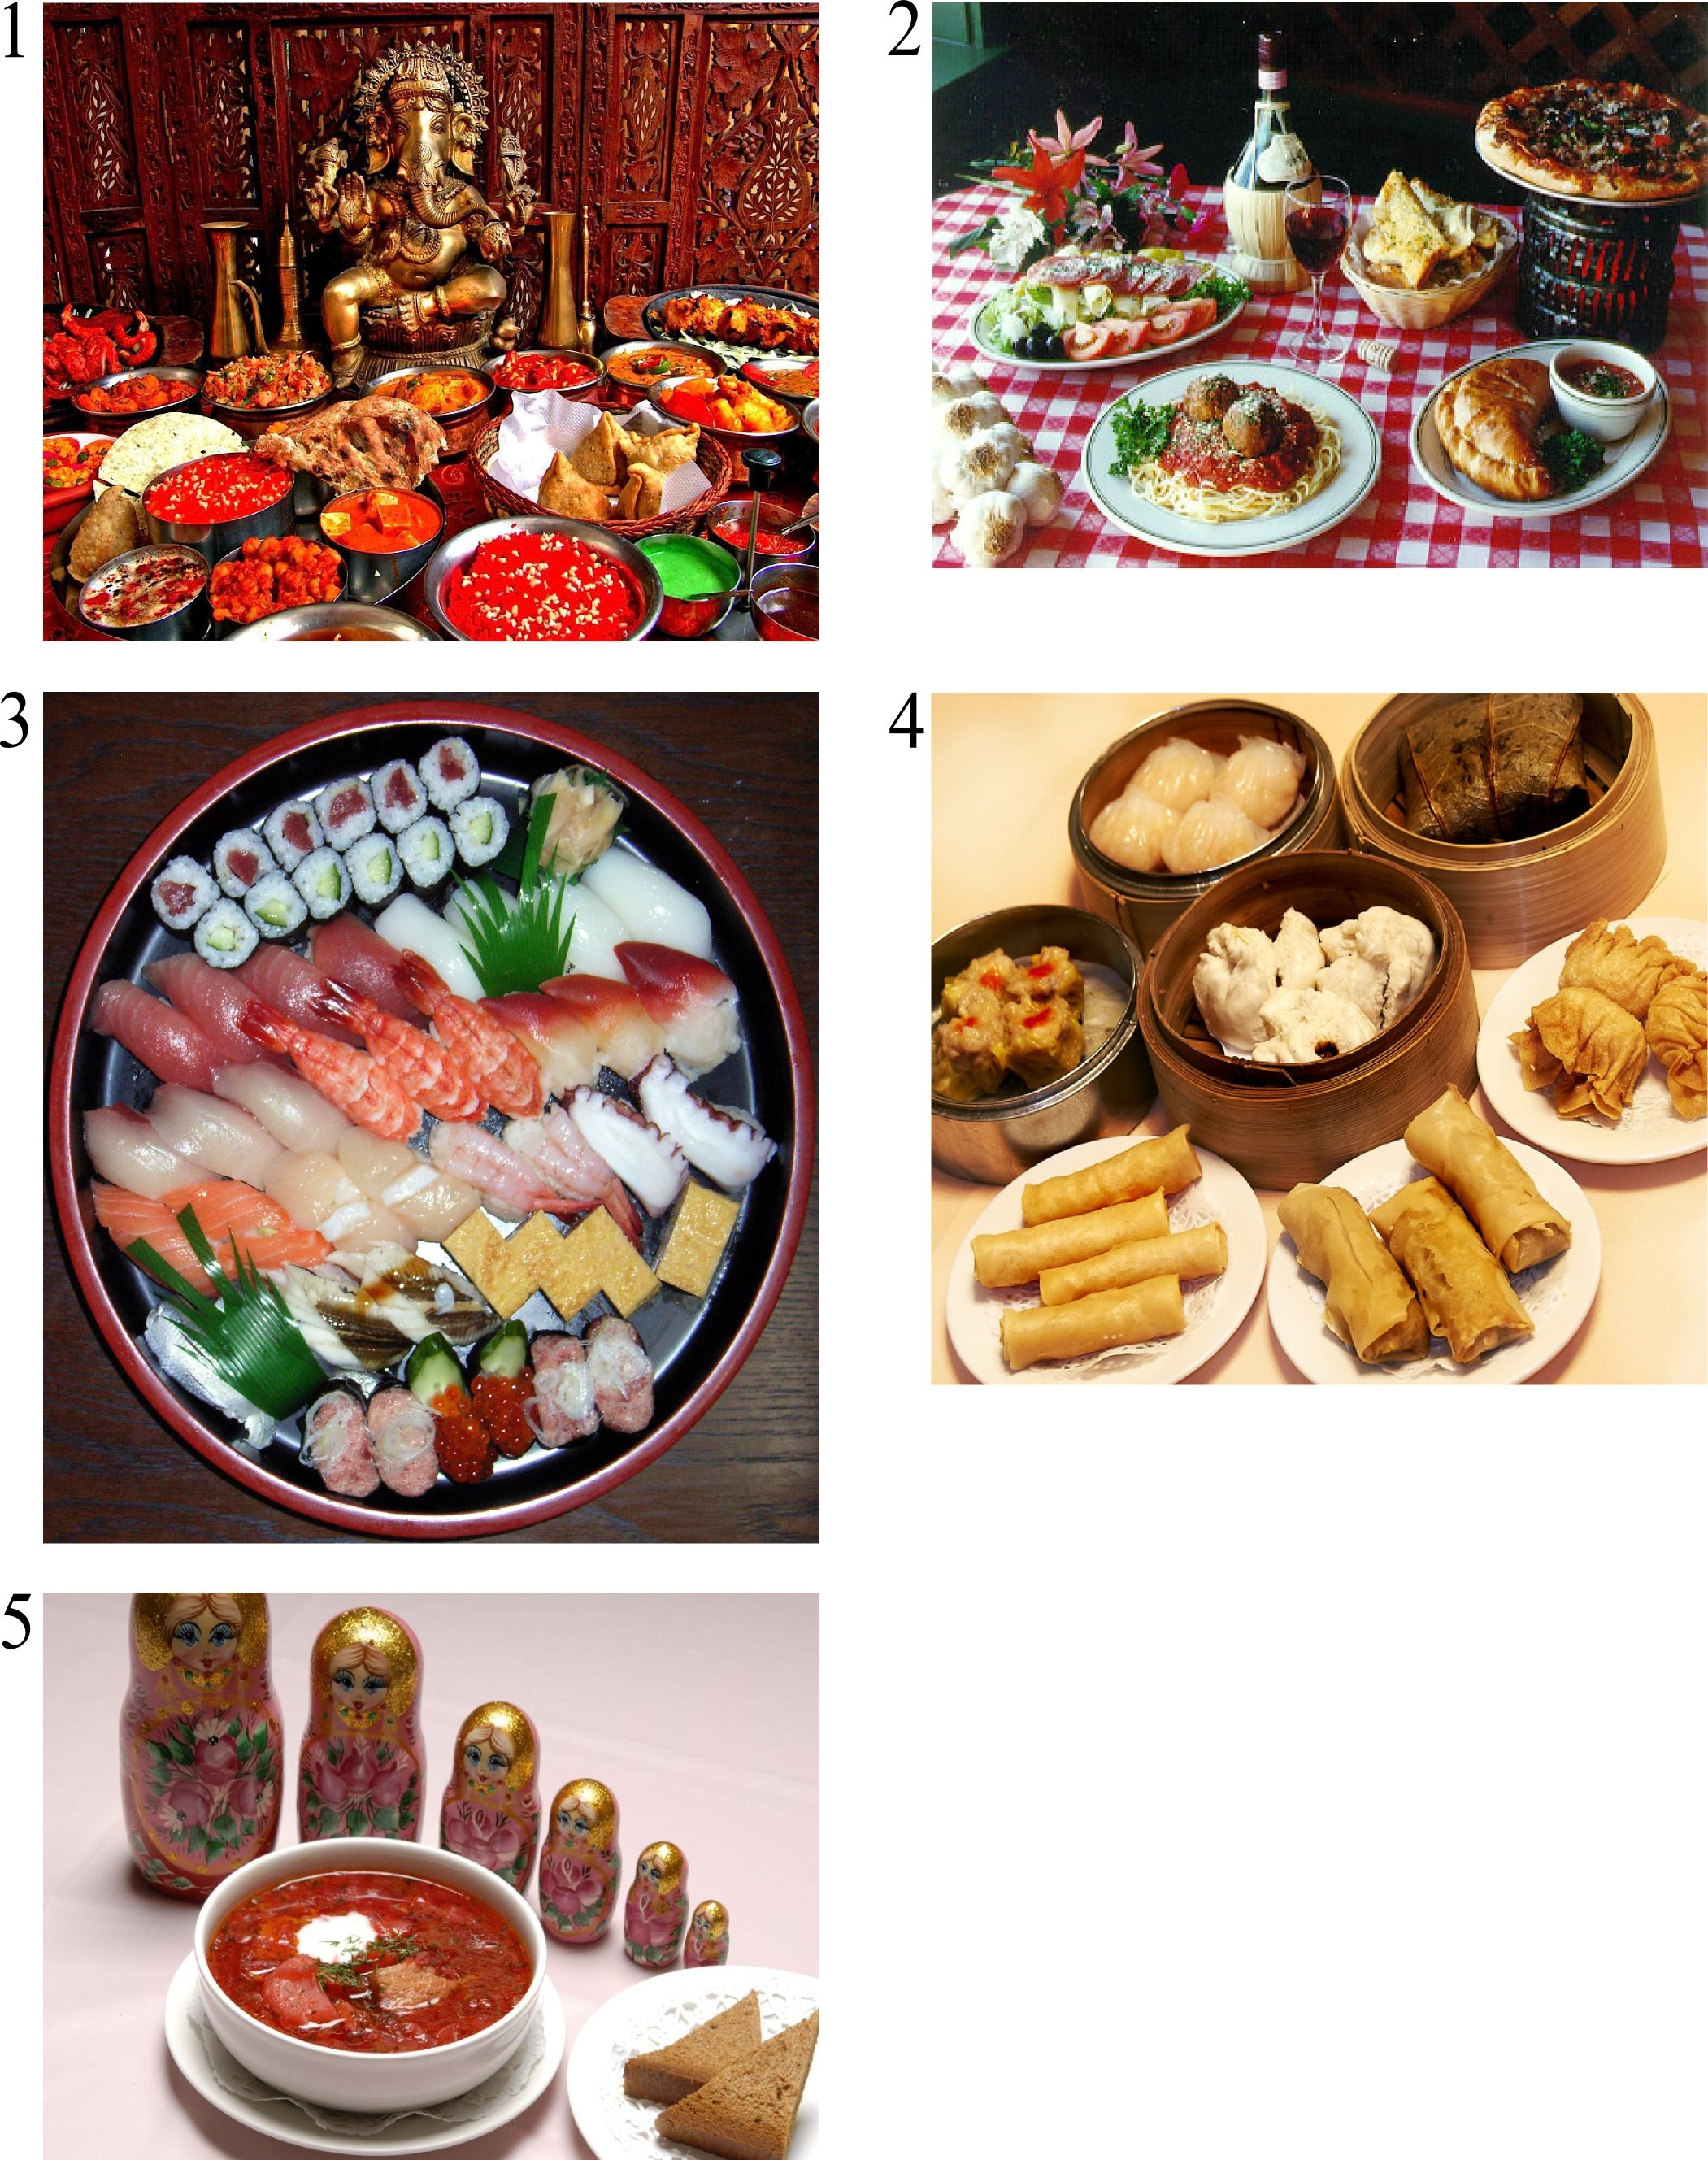
\includegraphics[scale=1.00]{../figs/taskImages/testImages.png}
	\caption{Testing image set. These images were presented to all workers in 
		the order shown after the priming set of images.}
\end{figure}

\begin{figure}
	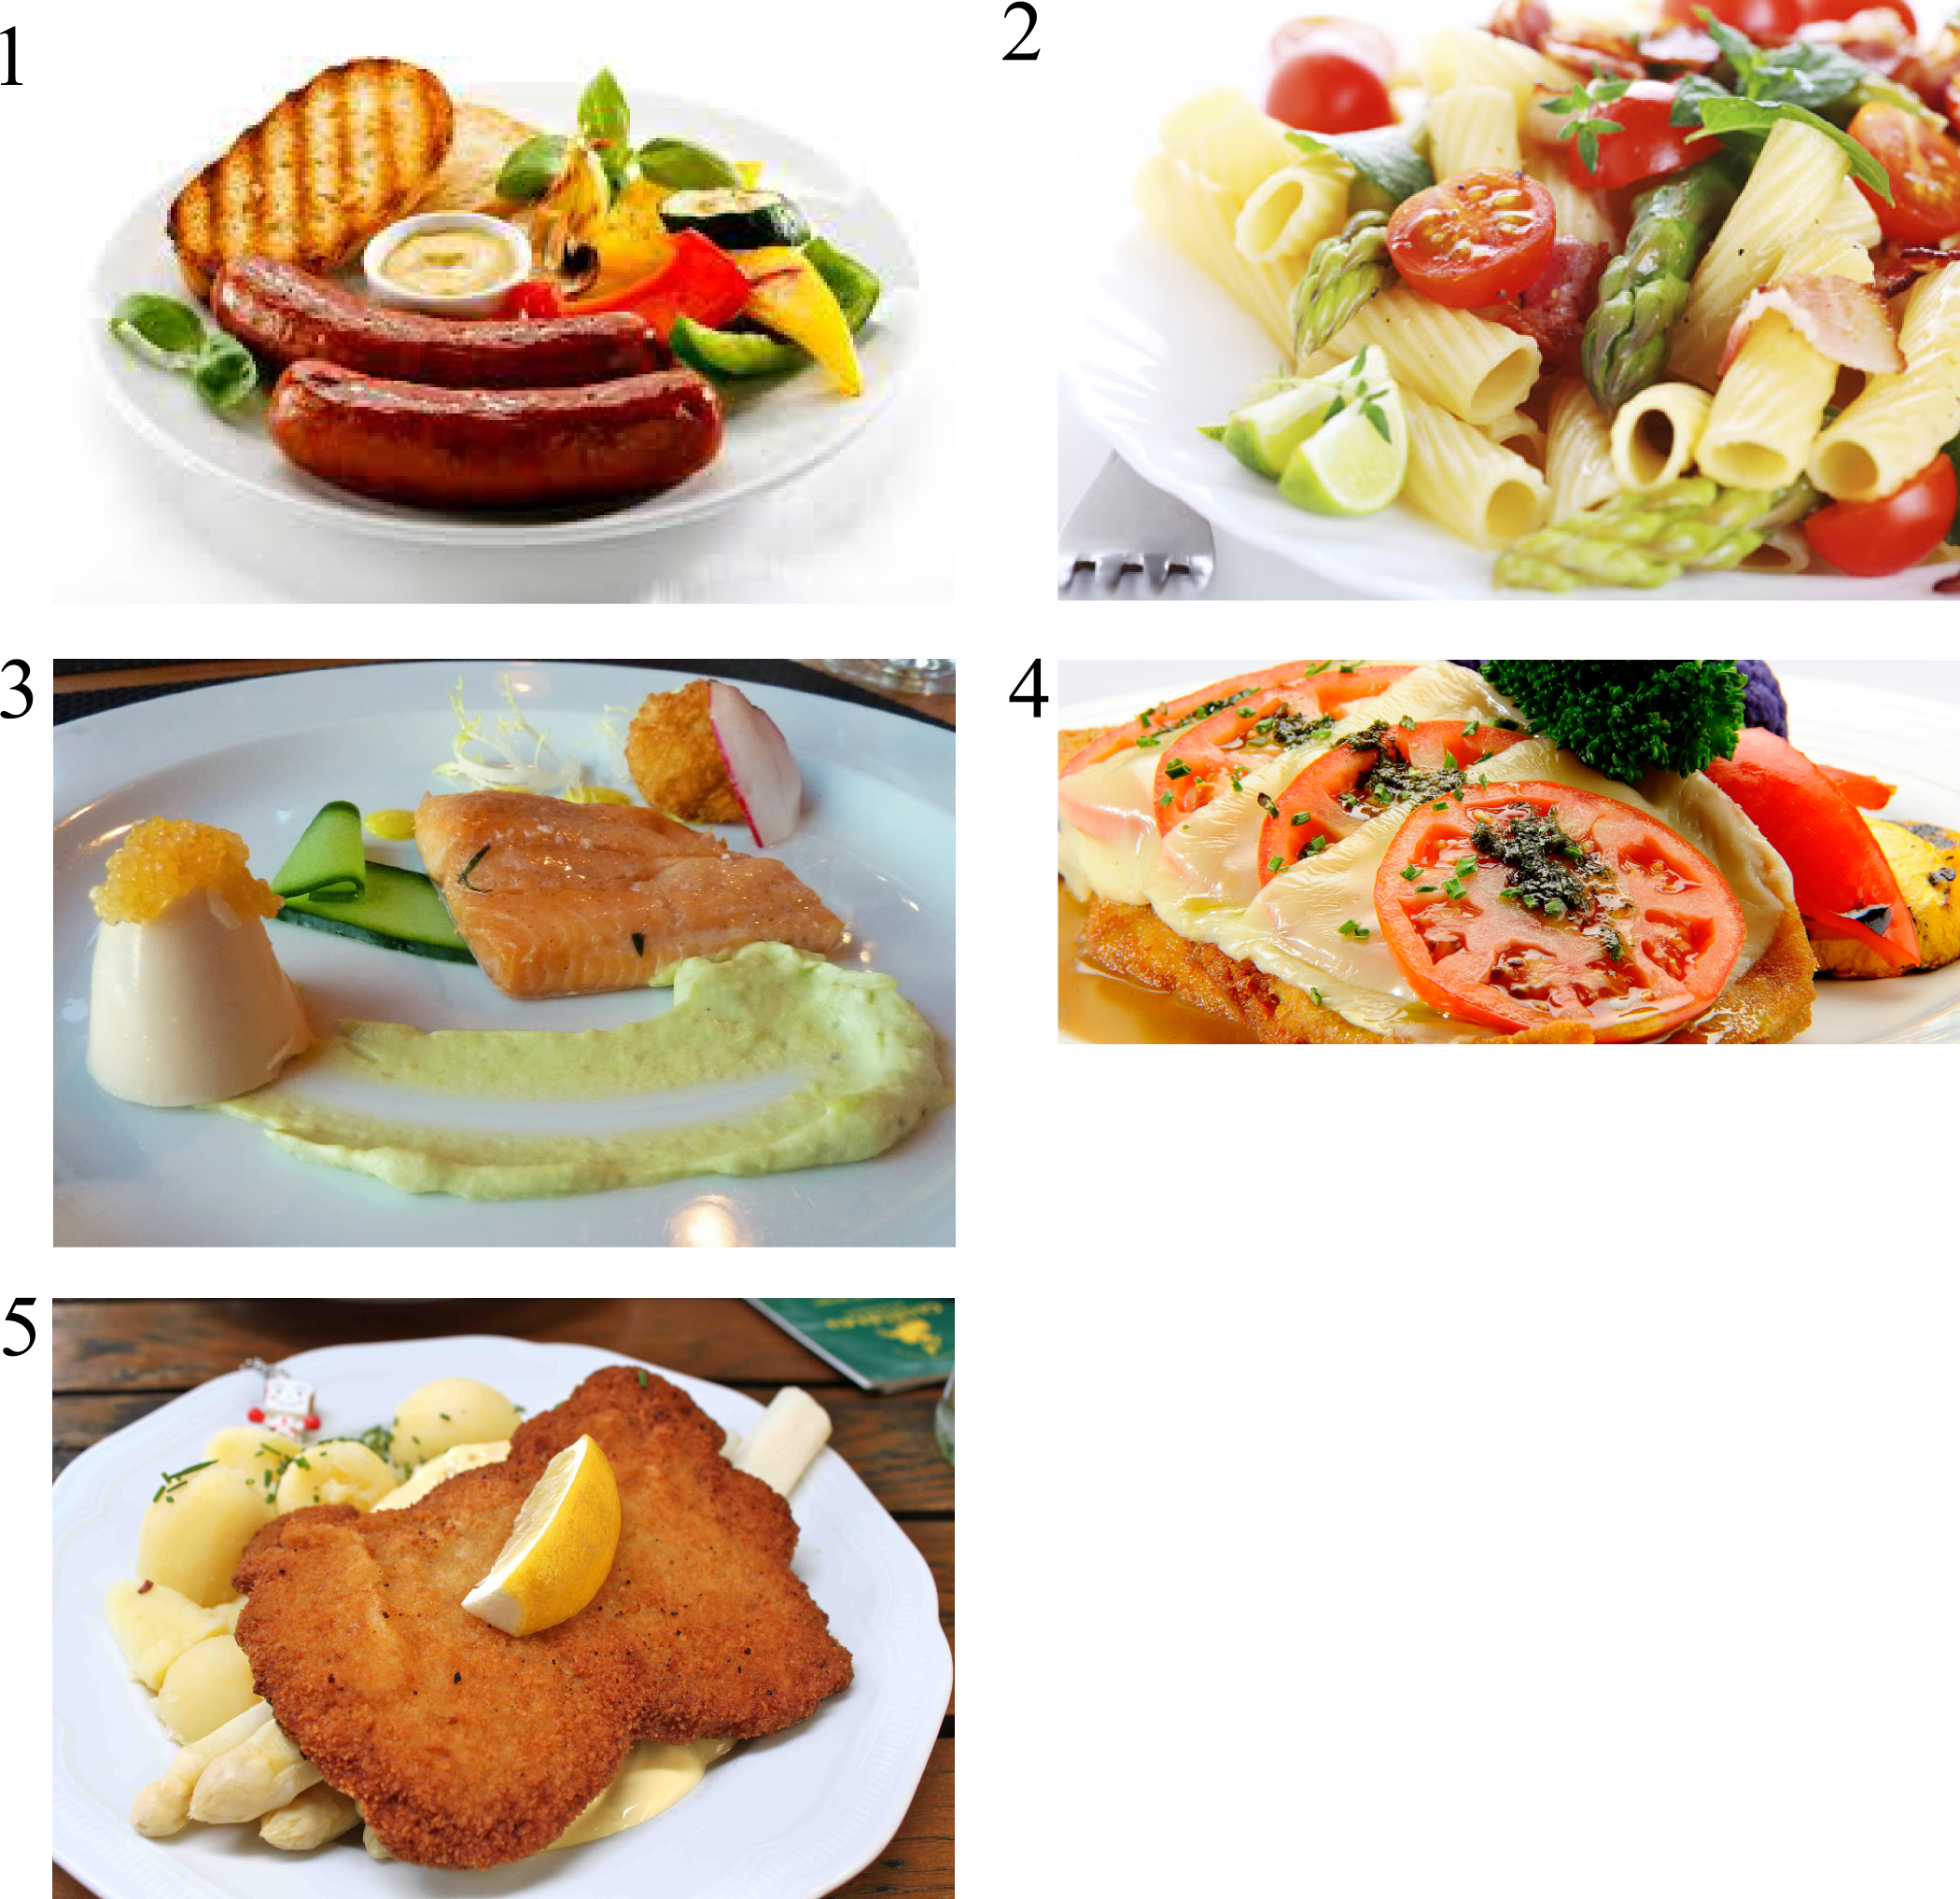
\includegraphics[scale=1.00]{../figs/taskImages/ambiguous.png}
	\caption{ Ambiguous image set. These images were presented to workers from 
		certain treatements (see \textbf{Table 1}) in the order shown.}
\end{figure}

\begin{figure}
	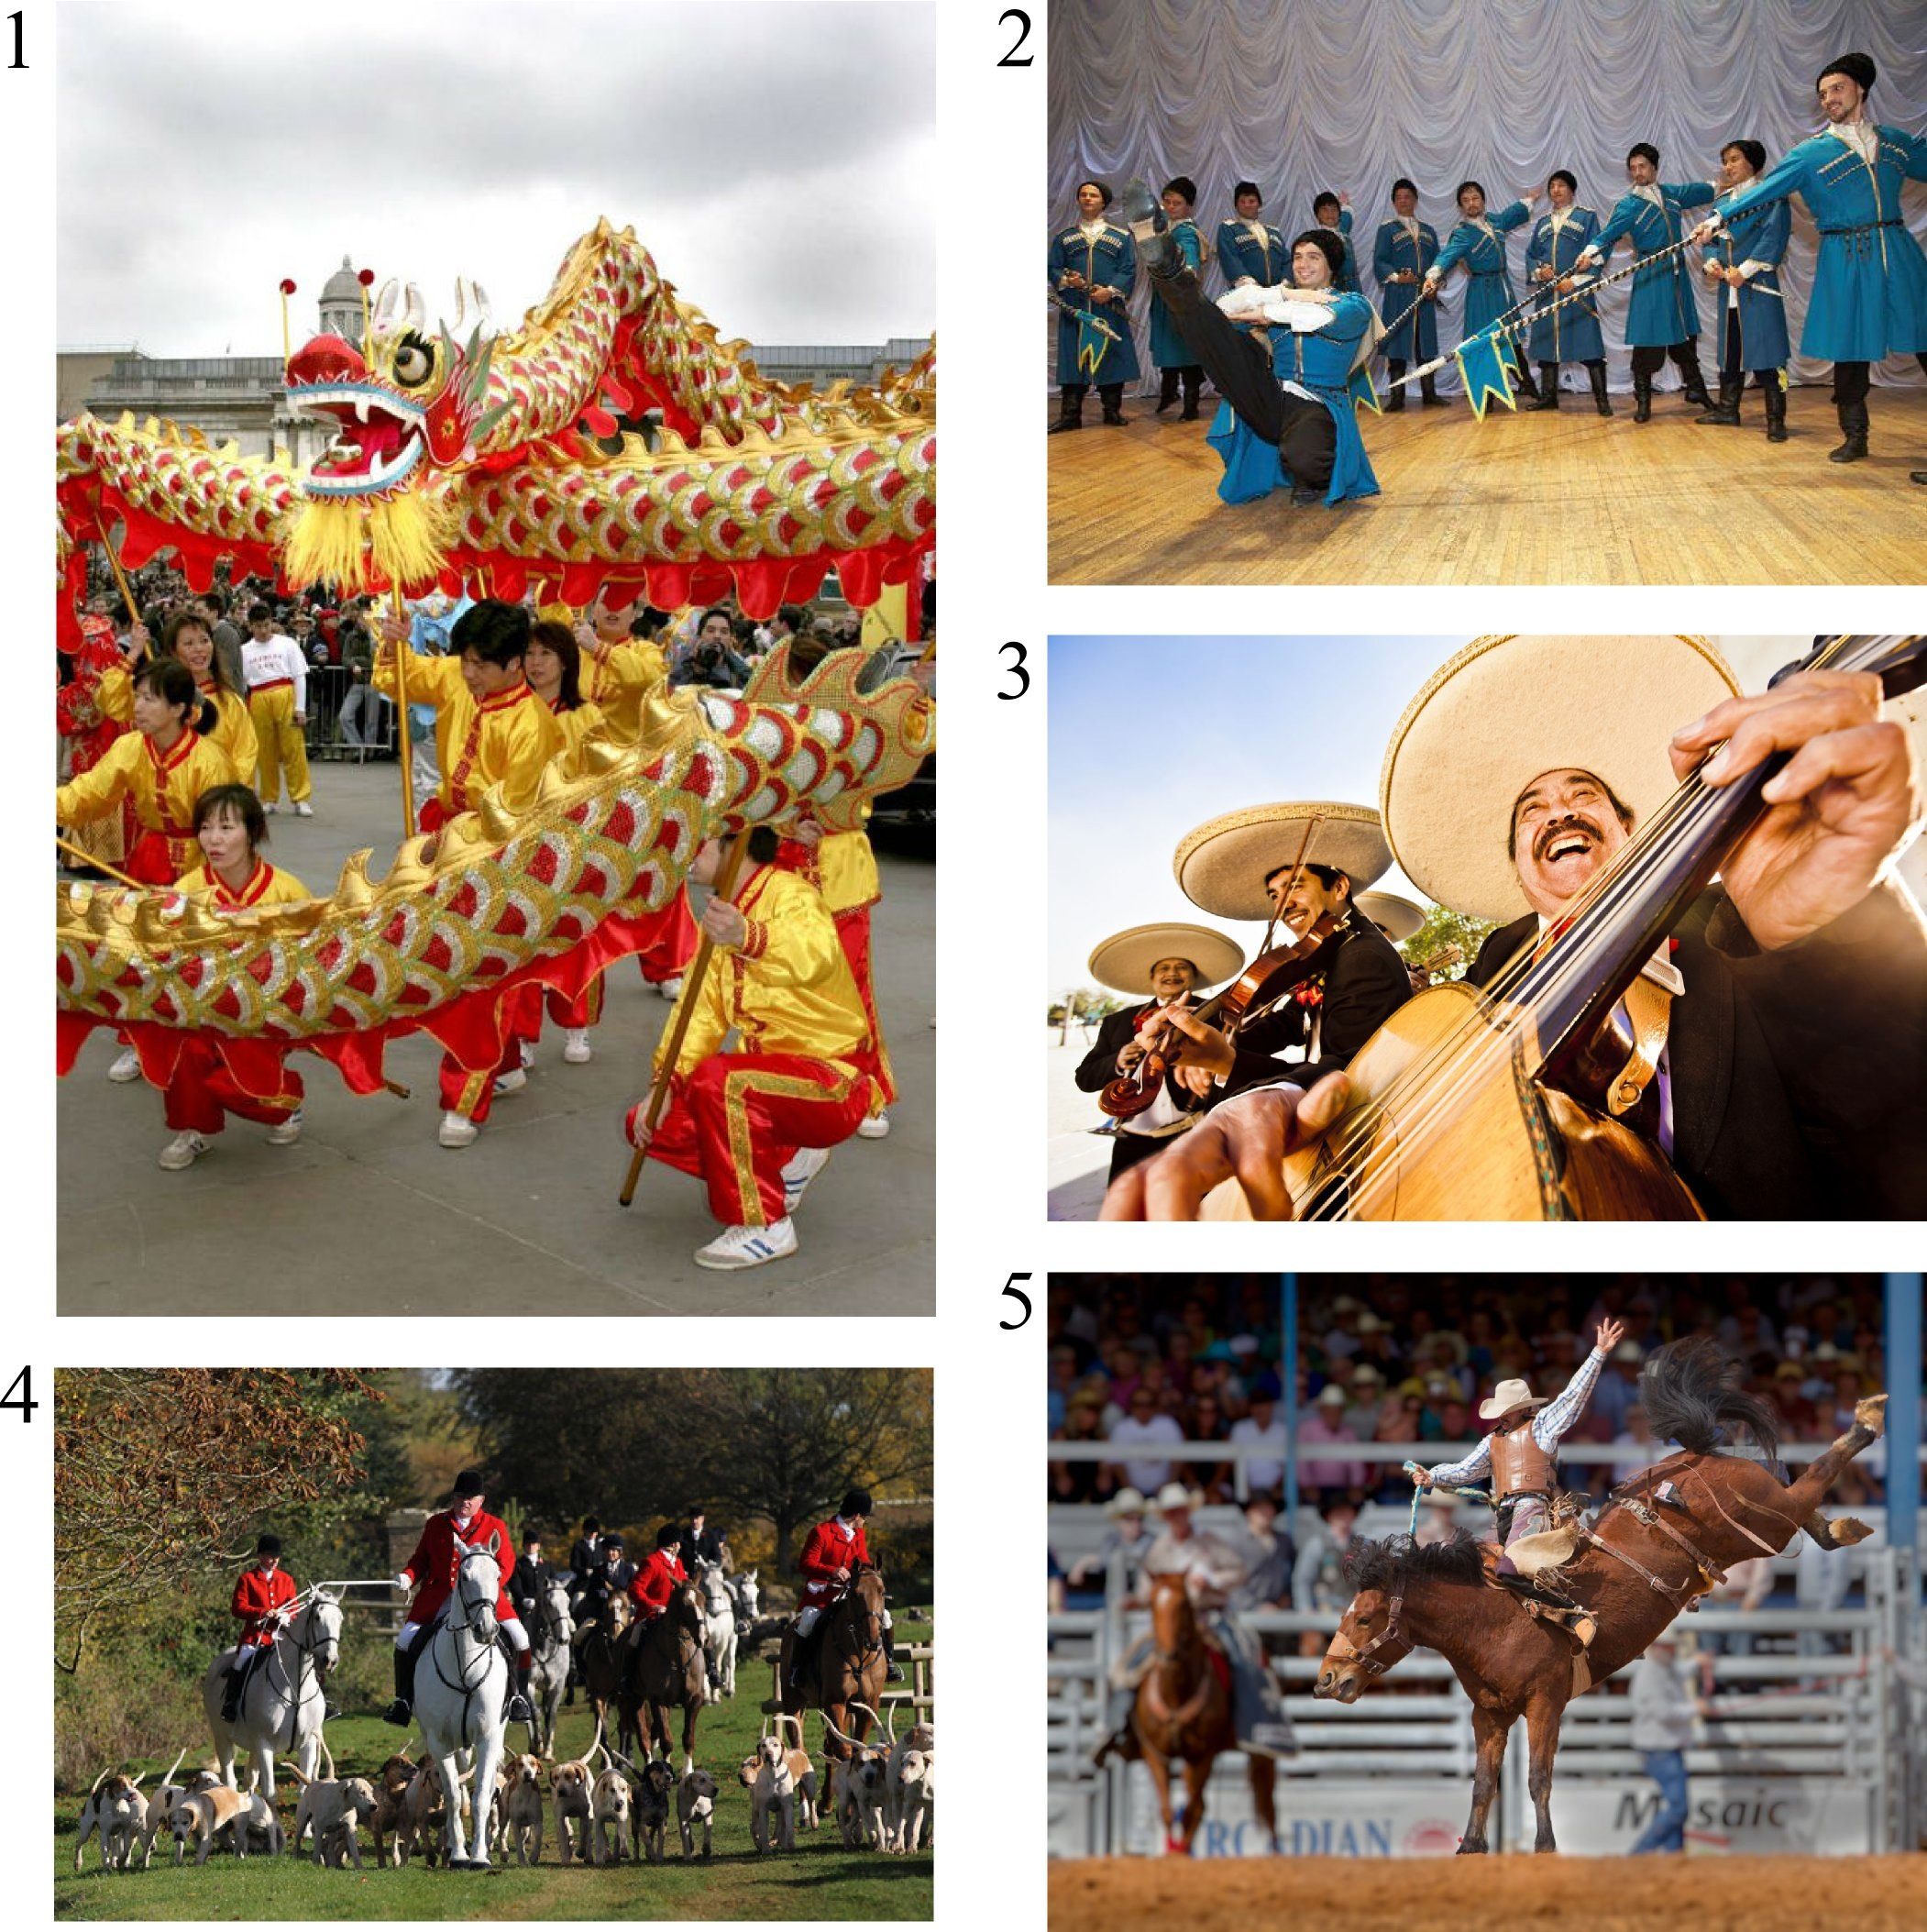
\includegraphics[scale=1.00]{../figs/taskImages/cultural.png}
	\caption{Cultural image set. These images were presented to workers from 
		certain treatements (see \textbf{Table 1}) in the order shown.}
\end{figure}

\begin{figure}
	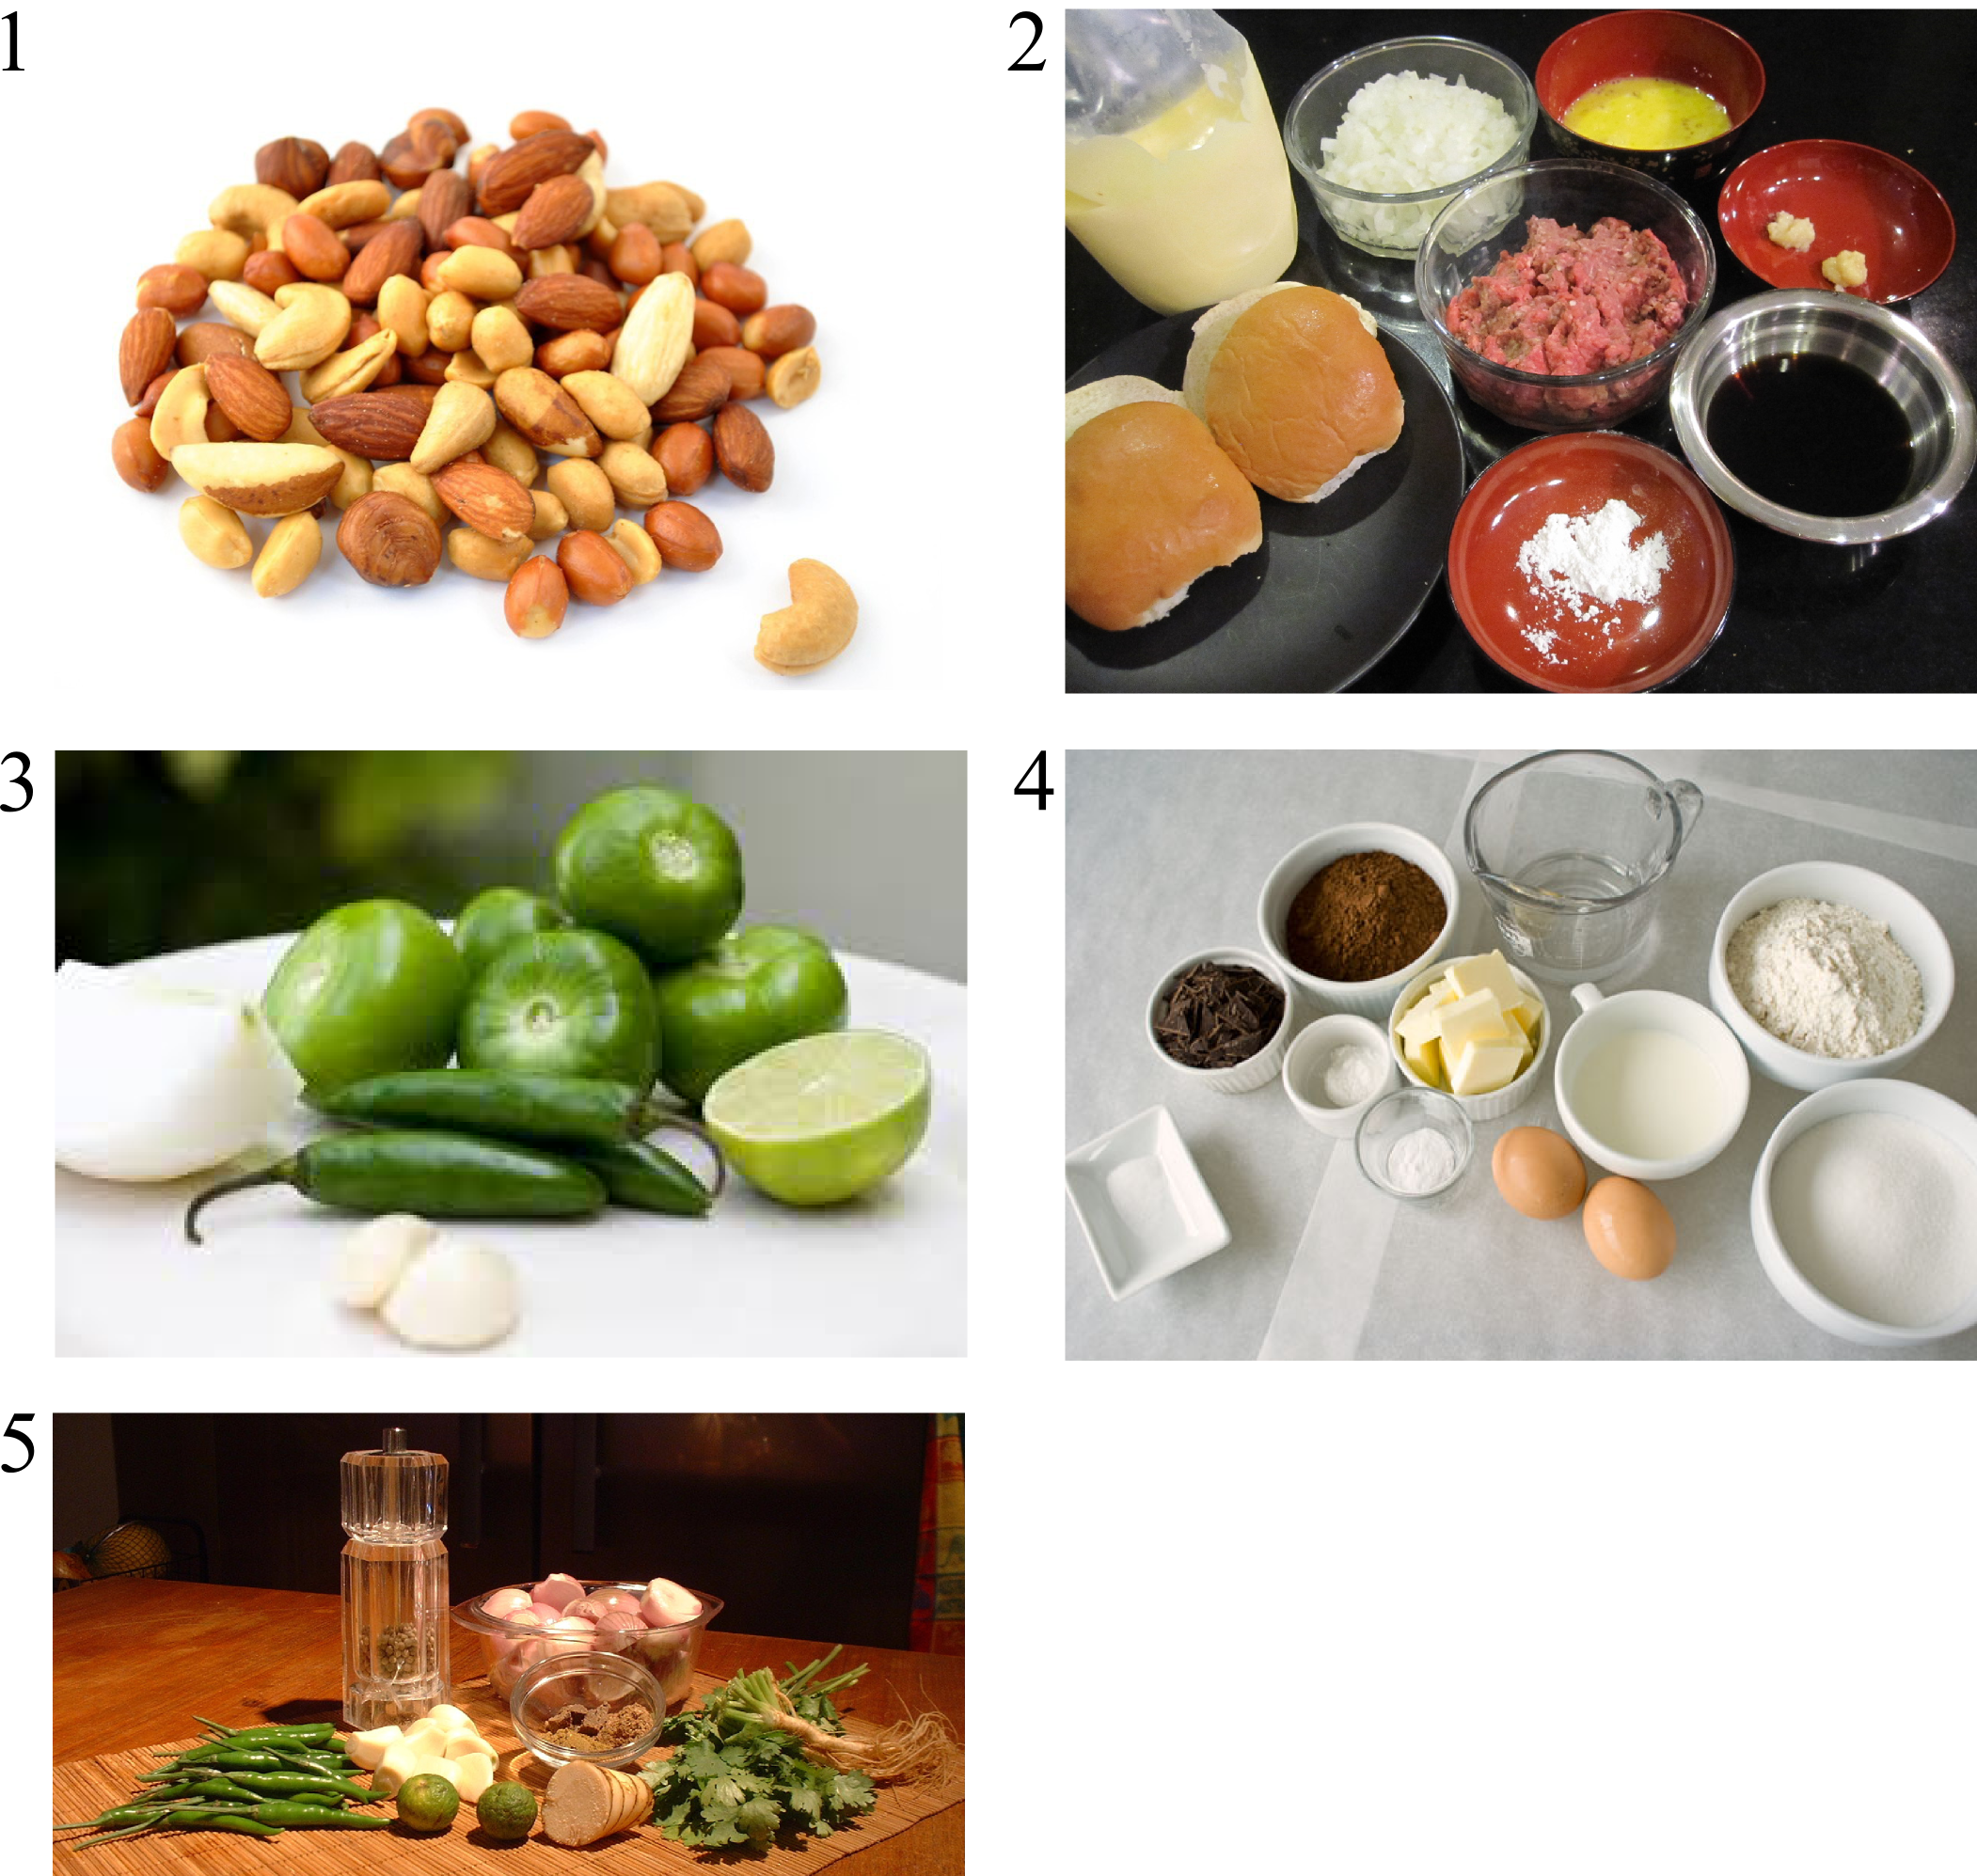
\includegraphics[scale=1.00]{../figs/taskImages/ingredients.png}
	\caption{ Ingredients image set. These images were presented to workers 
		from certain treatements (see \textbf{Table 1}) in the order shown.}
\end{figure}

\begin{figure}
	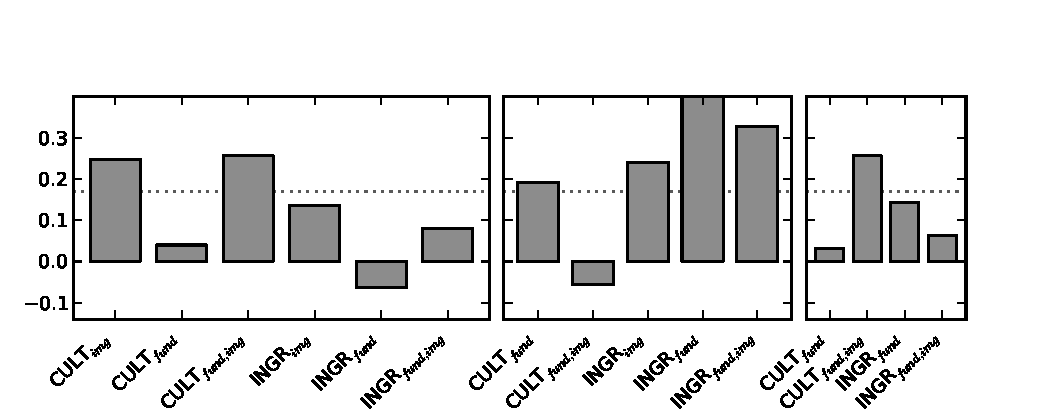
\includegraphics{../figs/f1-thetas.pdf}
	\caption{ $F_1$ score and $\theta_\text{NB}$ for the various 
priming treatments, as measured using a Naive Bayes classifier. Each panel 
presents classifier performance results that indicate the difference in
priming between a basis 
treatment, indicated in the inset, and the other treatments, indicated on the
abscissa. }
\end{figure}

\begin{figure}
	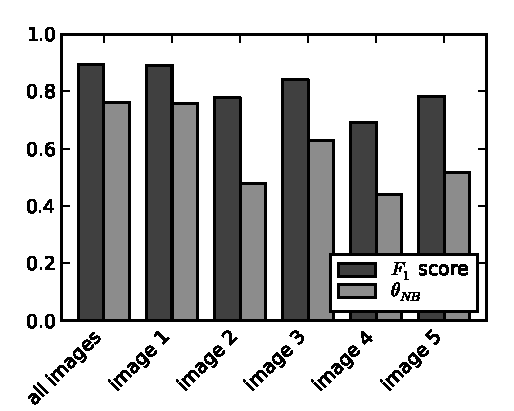
\includegraphics{../figs/longitudinalF1scores-t1-t2.pdf}
	\caption{ $F_1$ score and $\theta_\text{NB}$ for the classification of 
	$\textsc{cult}_{img}$ and $\textsc{ingr}_{img}$ using a Naive Bayes 
	classifier.  The classifier is provided only the labels attributed to
	particular images as indicated on the abscissa.}
\end{figure}

\begin{figure}
	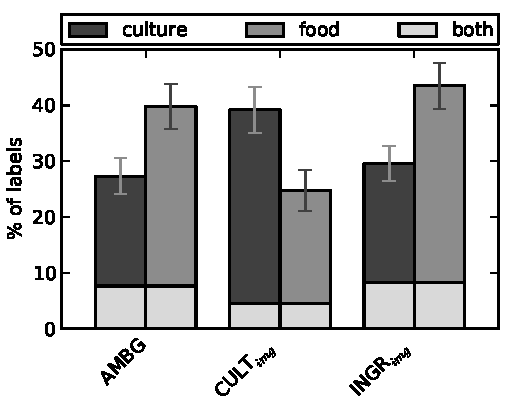
\includegraphics{../figs/orientationVsTreatment.pdf}
	\caption{Percent label composition (culture- vs food-oriented labels) for 
		various images and treatments.  Panel A shows the composition of 
		labels, aggregated over all treatments, as a function of test image.
		Panel B shows the composition of labels, aggregated over all images, as
		a function of treatment.  Panel C shows the composition of labels 
		attributed to the first test image by various treatments.}
\end{figure}

\begin{figure}
	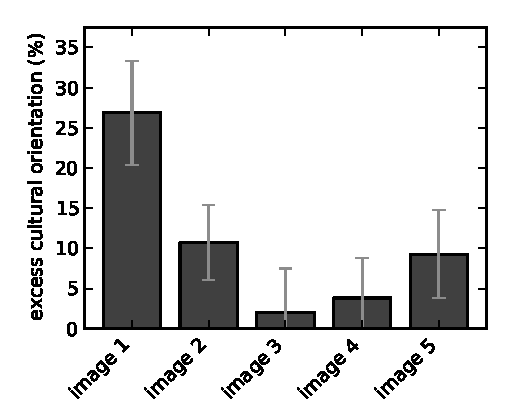
\includegraphics{../figs/excessCultureVsTreatment-t1.pdf}
	\caption{Excess culture-oriented label composition in the labels provided
		by $\textsc{cult}_{img}$ as compared to $\textsc{ambg}$, for various
		test images (see \textbf{Eq. 1} for calculation).
	}
\end{figure}

\begin{figure}
	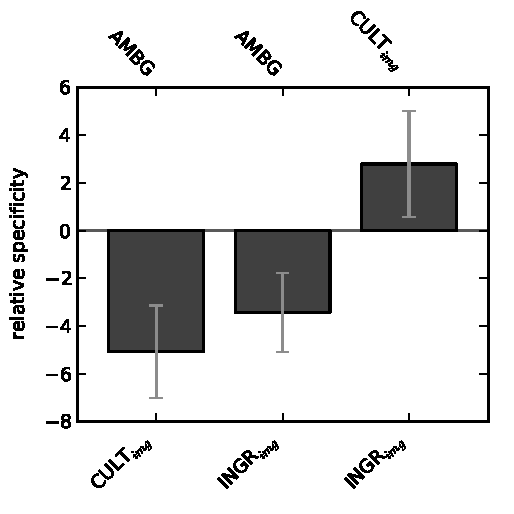
\includegraphics{../figs/specificity-allImages.pdf}
	\caption{Relative specificity of various treatments.
		Each panel shows the comparison between a basis treatment (inset) and 
		target treatments (abscissa).
		Bar heights indicate relative specificity of the target 
		treatment compared to the basis (a positive quantity means the target 
		is more specific), and are normalized to units of standard 
		deviations of the null comparison.  Dotted horizontal lines indicate
		the 95\% confidence interval for the null comparison, which necessarily
		has zero relative specificity (see \textbf{Methods} 
		for an explanation of the null comparison).  Panels D, E, and F 
		represent relative specificity calculated using only culture-oriented
		labels, while panels G, H, and I using only food-oriented labels.
		Labels that are both culture- and food-oriented are excluded from the
		calculations for panels D through I.
		}
\end{figure}

\begin{figure}
	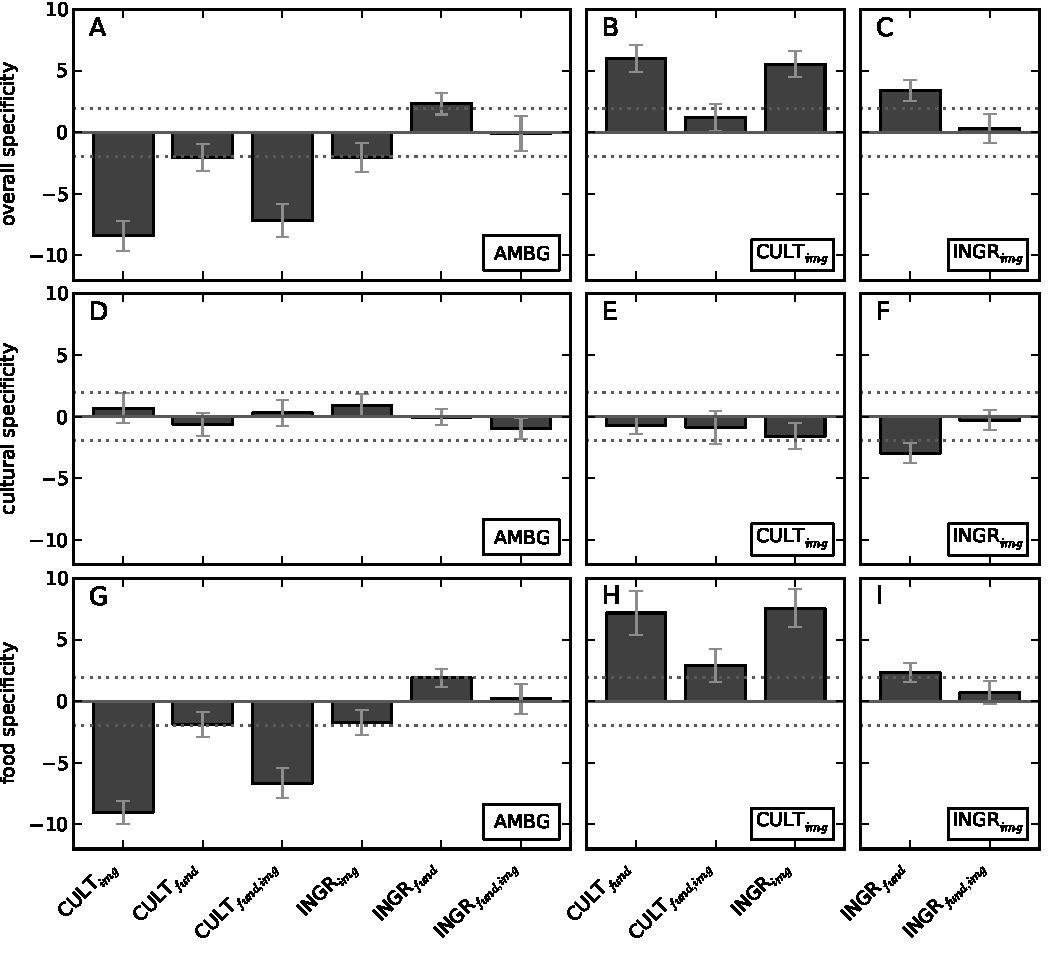
\includegraphics{../figs/specificity-test0.pdf}
	\caption{Relative specificity of various treatments, for labels attributed
		to the first test image.
		Each panel shows the comparison between a basis treatment (inset) and 
		target treatments (abscissa).
		Bar heights indicate relative specificity of the target 
		treatment compared to the basis (a positive quantity means the target 
		is more specific), and are normalized to units of standard 
		deviations of the null comparison.  Dotted horizontal lines indicate
		the 95\% confidence interval for the null comparison, which necessarily
		has zero relative specificity (see \textbf{Methods} 
		for an explanation of the null comparison).  Panels D, E, and F 
		represent relative specificity calculated using only culture-oriented
		labels, while panels G, H, and I using only food-oriented labels.
		Labels that are both culture- and food-oriented are excluded from the
		calculations for panels D through I.
		}
	\end{figure}

\end{document}


